\newpage
\section {Билет 15. Модели взаимодействия, ошибок, безопасности.}

Различные архитектуры распределённых систем имеют много общего.\\
\\
\textbf{1. Модели взаимодействия}
\begin{itemize}
\item Характеристики коммуникационного канала:

Основные характеристики это:

\hspace{-6px}\textit{Пропускная способность} - сколько гбит можно передать за единицу времени.

\hspace{-6px}\textit{Задержка} - сколько времени уходит на передачу сообщения, зависит от физической структуры и количества промежуточных структур.

\hspace{-6px}\textit{jitter} - изменение величины задержки при передаче последовательности пакетов, то есть существует некоторая средняя задержка, но каждый конкретный пакет передается быстрее или медленнее. Каким-то приложениям оптимизация jitter важна, каким-то нет, например при скачивании web страницы, он не важен, а в мультимедийном приложении будет важен. Один из вариантов оптимизации jitter-а в случае показа видео, может быть допущение потери пакетов, так как небольшую их потерю пользователь не заметит, а задержки во время показа, более ощутимы и проблематичны.

\item Упорядочивание сообщений (причинно-следственный порядок).

Мы можем спокойно сравнивать время события в одном процессе, но между разными процессами их можно сравнивать только при наличии передачи сообщения, используя то, что нельзя получить сообщение раньше, чем оно было отправлено.

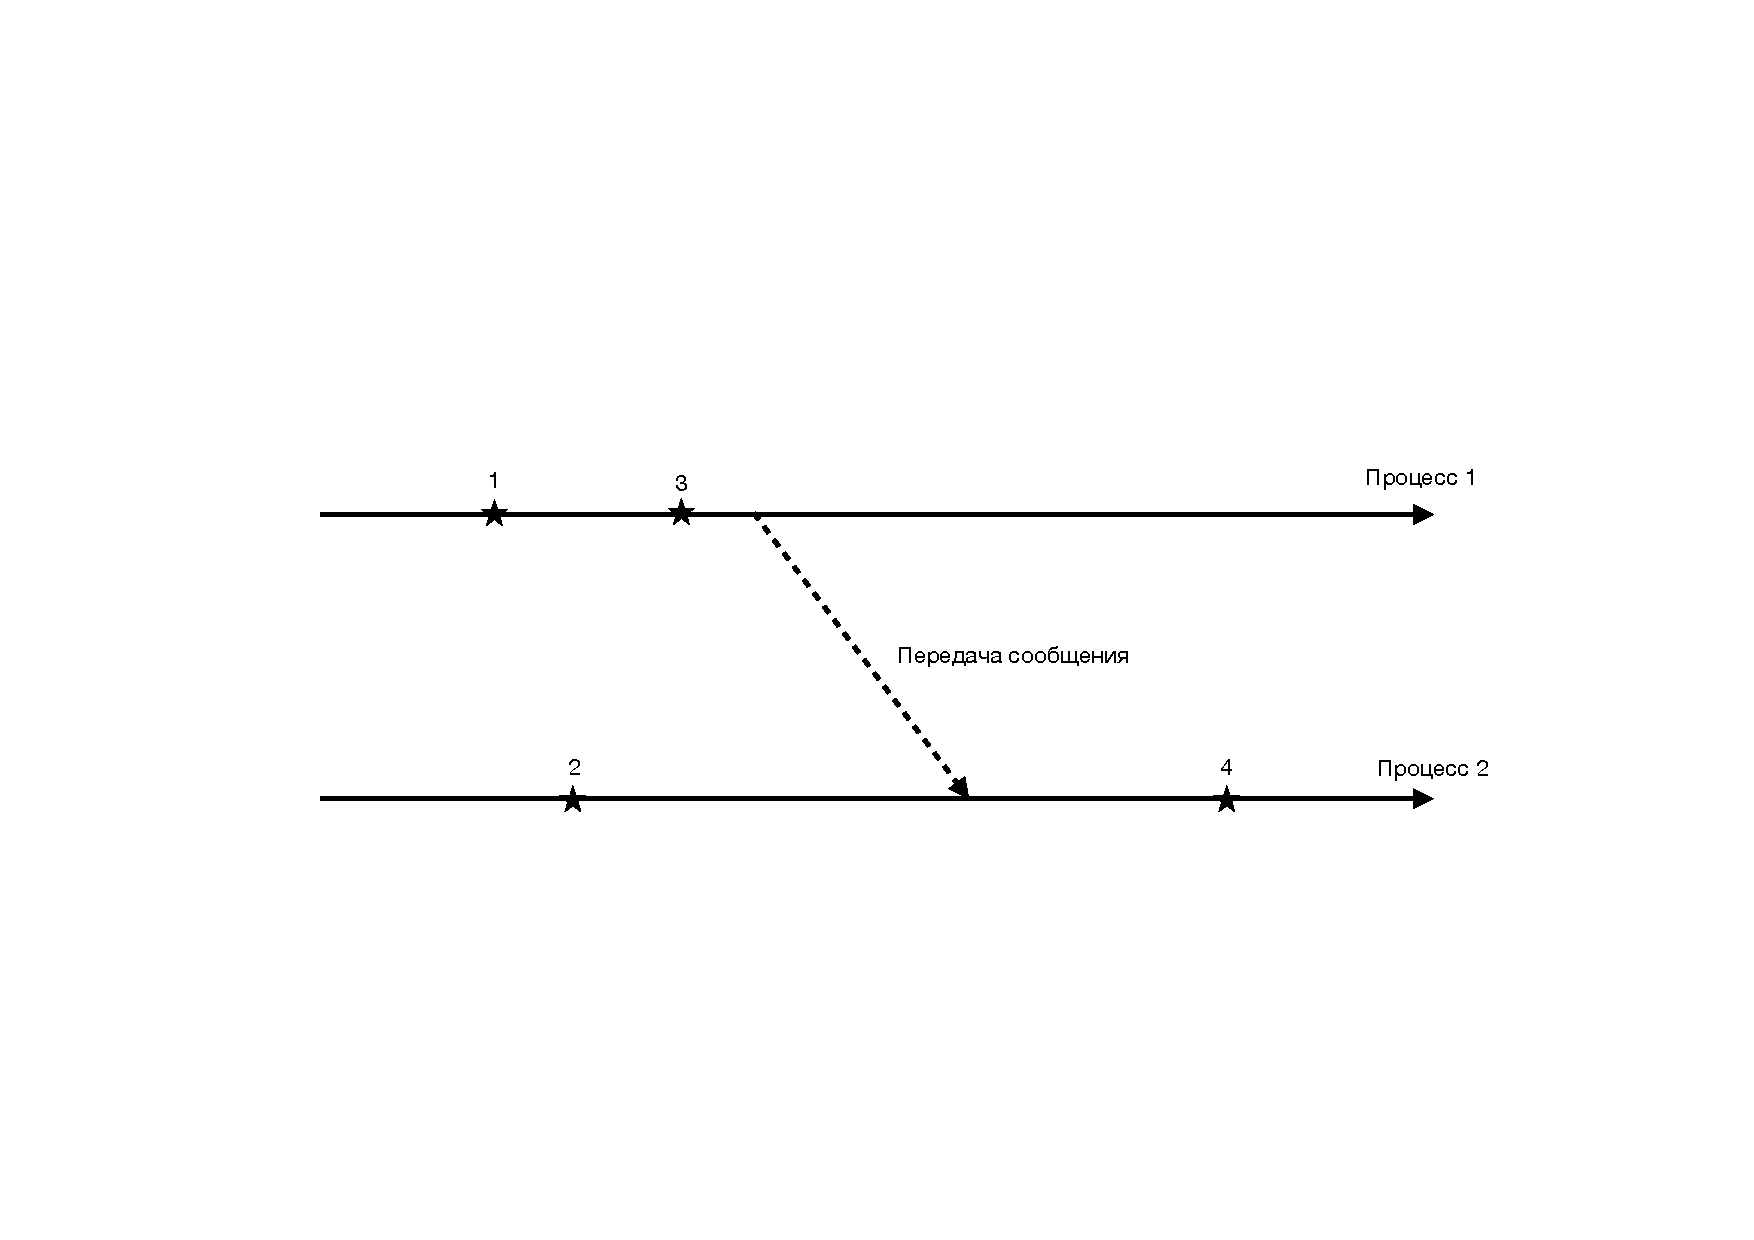
\includegraphics[scale=0.7]{15/masseg_time.pdf}

Так, на картинке, процесс 2 знает порядок временных меток в процессе 1 до передачи сообщения (1 и 3) и знает что они все были до метки 4, но сравнить порядок 1 или 3 с меткой 2 нельзя, так в распределённой системе отсутствуют глобальные часы и синхронизировать раз и на всегда процессы нельзя.
 
\textit{Более подробно этот пункт разобран в билете \ref{b20}.}
 
\item  Синхронные и асинхронные системы.

\hspace{12px}В \textit{синхронной системе} предполагается, что каждое сообщение будет доставлено в течение некоторого заданного времени (если пакет не был доставлен за какое-то время, то он не будет доставлен никогда), а также известно время ответа любого другого узла (время выполнения операций).
Это позволяет пользователям моделировать протокол с фиксированной верхней границей, т.е. со значением максимального времени, требуемого на доставку сообщения принимающей стороне.

\hspace{12px}В \textit{асинхронной системе} предполагается, что сеть может произвольно задерживать сообщения на любой период времени, дублировать их или менять их порядок. Другими словами, фиксированная верхняя граница времени, необходимого на отправку и получение сообщения, отсутствует.

\hspace{12px} Асинхронная система менее удобная, но более распространённая в реальных распределённых системах, так как обычно компьютеры могут выходить из строя или уходить в автономный режим, а сообщения могут удаляться, дублироваться, задерживаться или поступать в произвольном порядке из-за проблем сети.
\end{itemize} 
\textbf{\noindent 2. Модели ошибок}

Отказ какого-то процесса может быть двух типов:
\begin{itemize}
\setlength\itemsep{0.0001em}
\item \textit{Наблюдаемый отказ}  -  другие участники могут узнать, что он погиб.
\item \textit{Ненаблюдаемый отказ}  - другие участники не могут узнать, что он погиб. Такие отказы более распространённые, поэтому, когда в алгоритме нужно найти гарантированно "живой" процесс, его часто ищут на основе таймеров, то есть если какой-то процесс не отвечает, то он начинает подозреваться в отказе.
\end{itemize}

Также ошибки могут быть следующих типов:\\
\textit{Потеря} (в канале) - сообщение отправлено, но не дошло. \\
\textit{Пропуск отправки} (в процессе) - процесс не отправляет сообщения.\\
\textit{Пропуск приема} (в процессе) - процесс не получает сообщения.\\
\textit{Произвольное или византийское поведение} (и в канале, и в процессе) - поведение, не предписанное протоколом, возникшее из-за ошибок или же злоумышленно.\\
\\
\newpage
\textbf{\noindent 3. Модели безопасности}

Политика информационной безопасности - документ на естественном языке

Модель информационной безопасности - формализация этой политики, то есть выражение утверждений, написанных на русском языке, в терминах какого-то формального языка, а также реализация этой модели в распределённой системе. \\

В модели безопасности должны быть определенны:
\begin{itemize}
\item Описание информационной системы
\item Структурно-функциональные характеристики
\item Описание угроз безопасности
\item Модель нарушителя
\item Возможные уязвимости
\item Способы реализации угроз
\item Последствия от нарушения свойств безопасности информации.
\end{itemize}




